

\begin{figure}
  \centering
  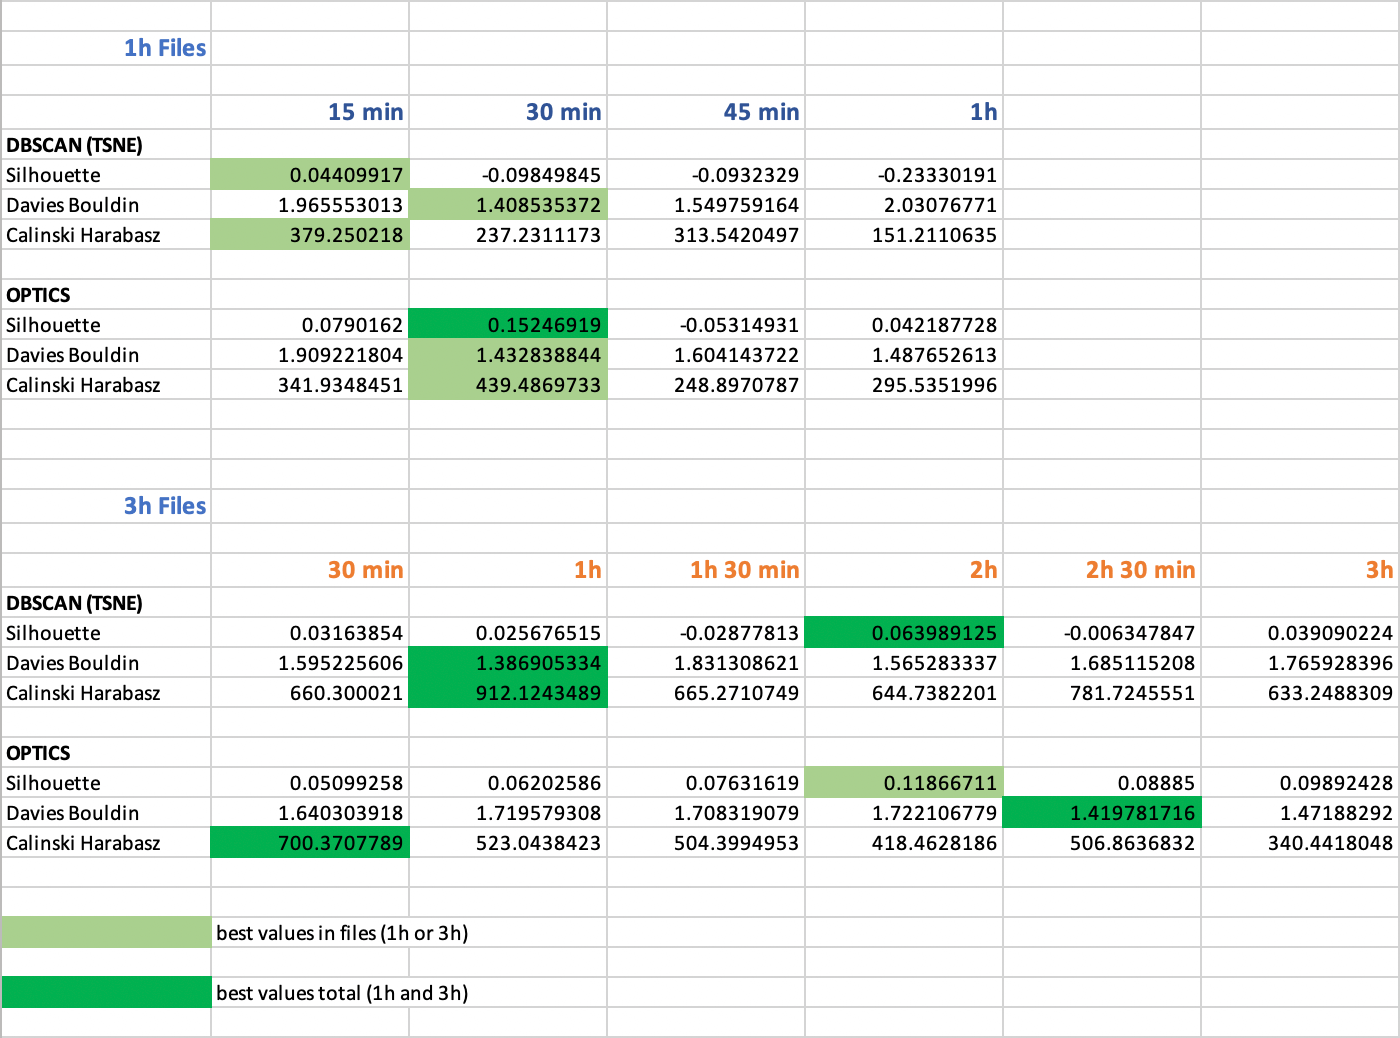
\includegraphics[width=0.8\textwidth]{./images/clusteringResults/clusteringResults1.png}
  \caption{Evaluation scores comparison from 1h run of t-SNE and clustering with a learning rate of 20.}
  \label{figure:clusteringResults1}
\end{figure}

\begin{figure}
  \centering
  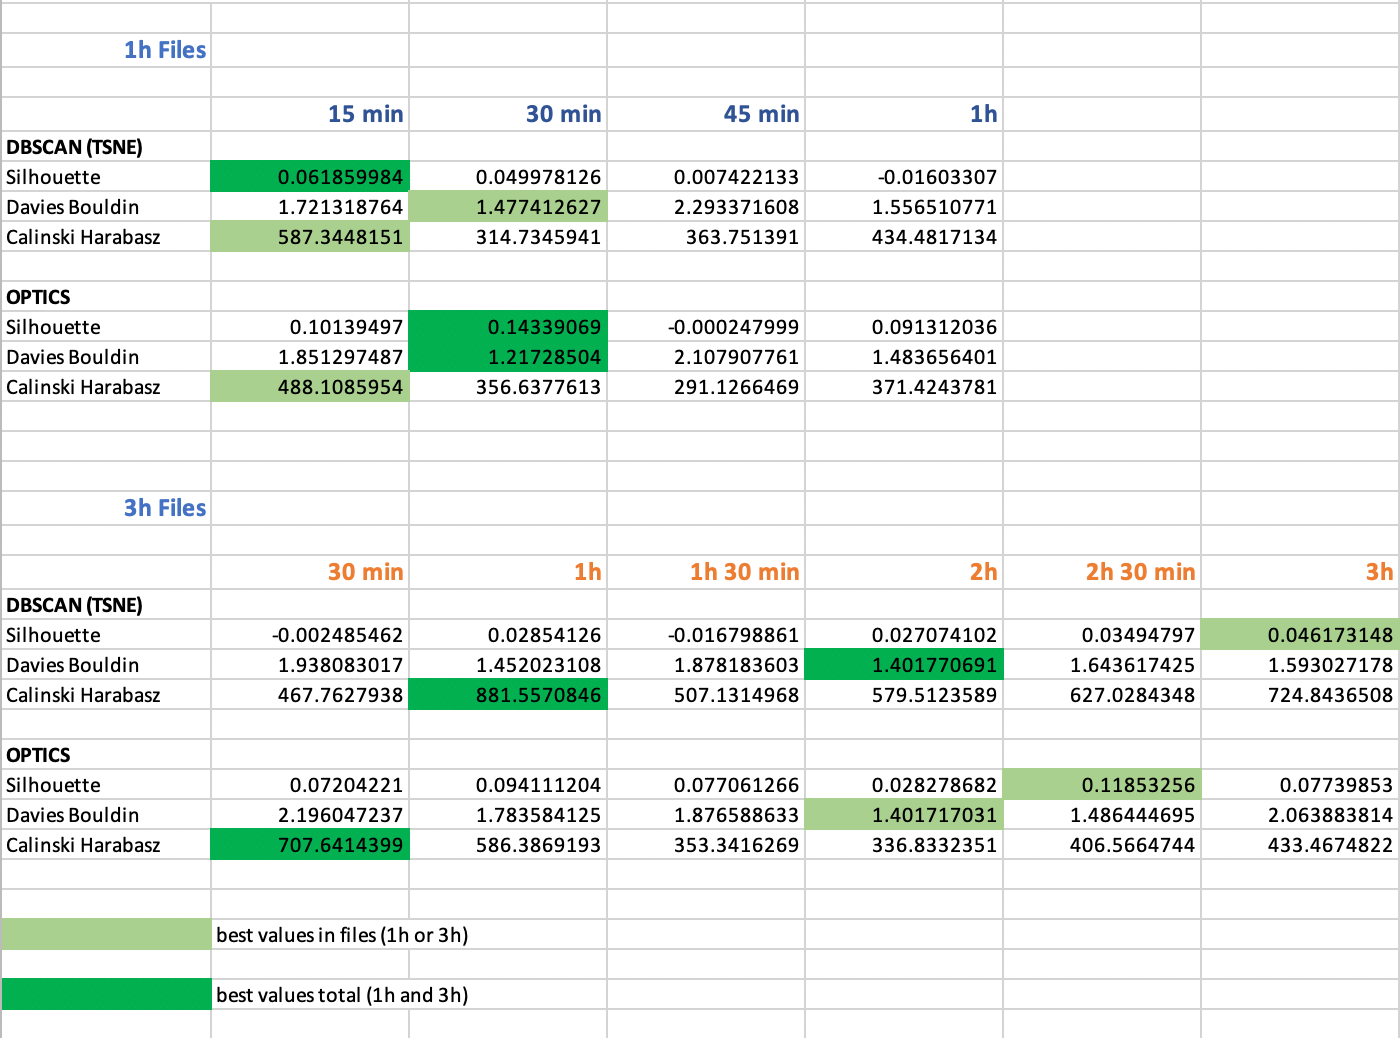
\includegraphics[width=0.8\textwidth]{./images/clusteringResults/clusteringResults2.png}
  \caption{Evaluation scores comparison from 1h run of t-SNE and clustering with a learning rate of 20.}
  \label{figure:clusteringResults2}
\end{figure}


\begin{figure}
  \centering
  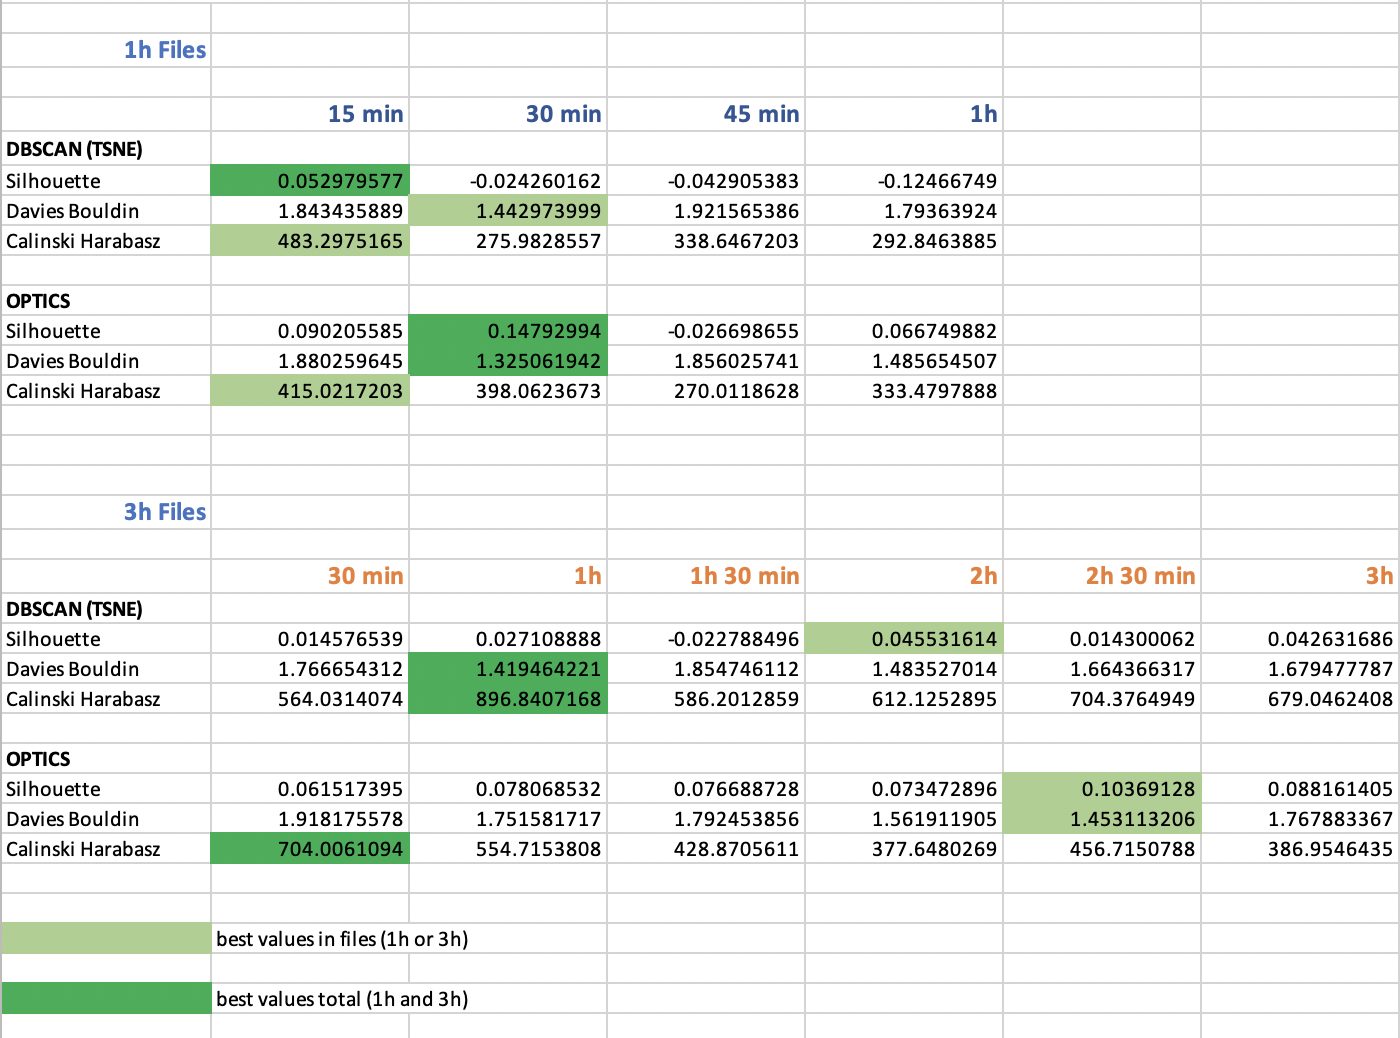
\includegraphics[width=0.8\textwidth]{./images/clusteringResults/clusteringResults3.png}
  \caption{Evaluation scores comparison averaged from figures \ref{figure:clusteringResults1} and \ref{figure:clusteringResults2}}
  \label{figure:clusteringResults3}
\end{figure}

\begin{figure}
  \centering
  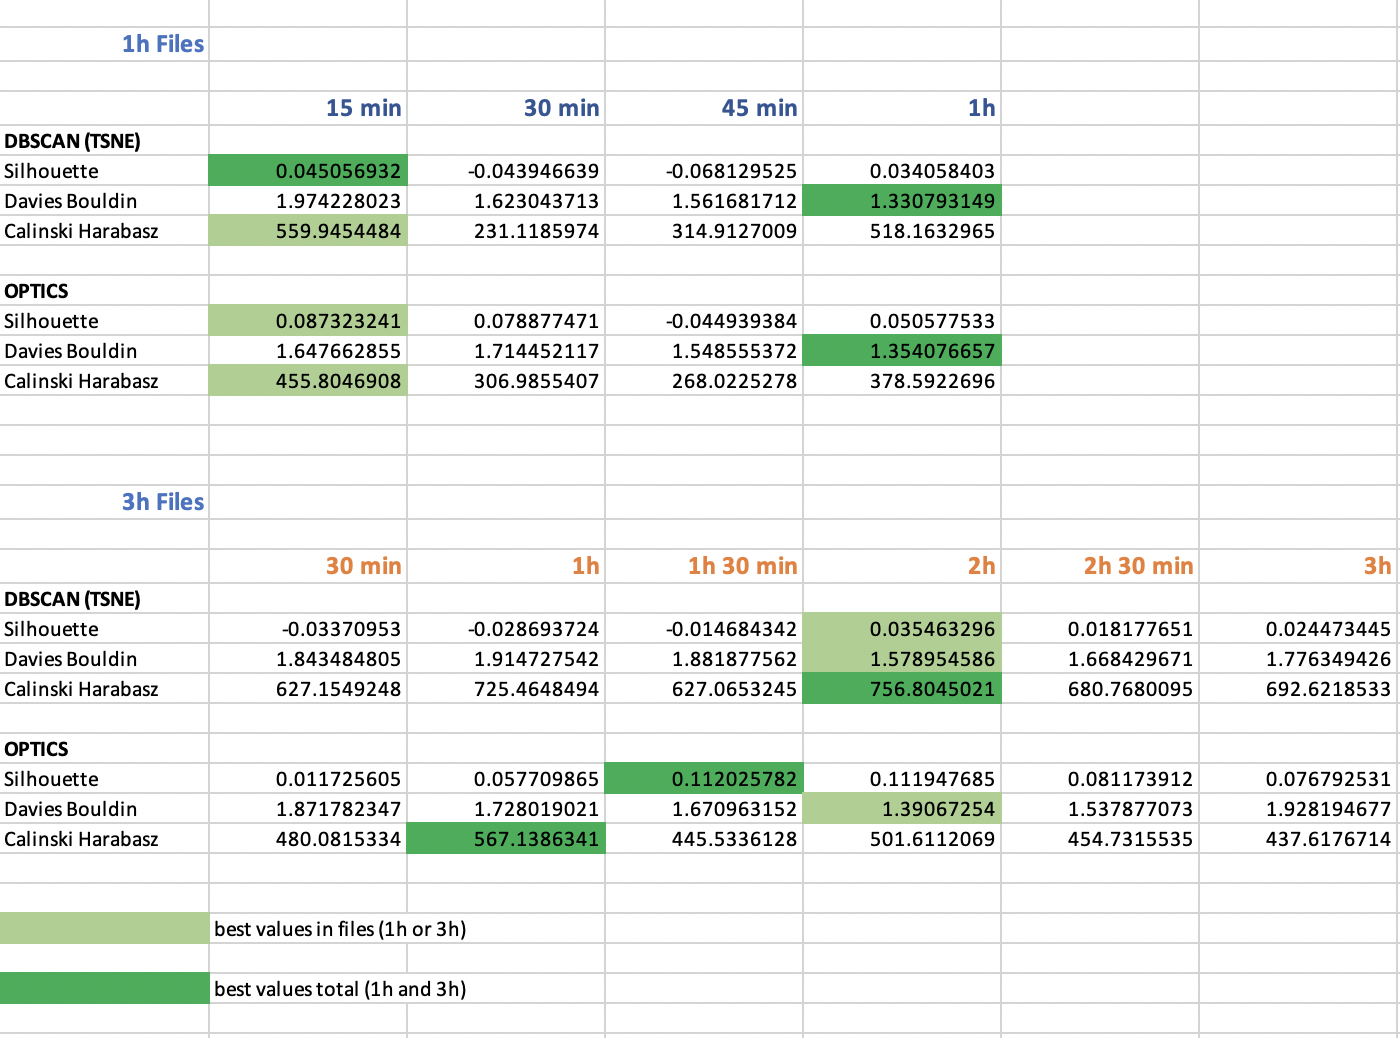
\includegraphics[width=0.8\textwidth]{./images/clusteringResults/clusteringResults4.png}
  \caption{Evaluation scores comparison averaged from 2 runs of t-SNE and clustering with a learning rate of 20.}
  \label{figure:clusteringResults4}
\end{figure}

\begin{figure}
  \centering
  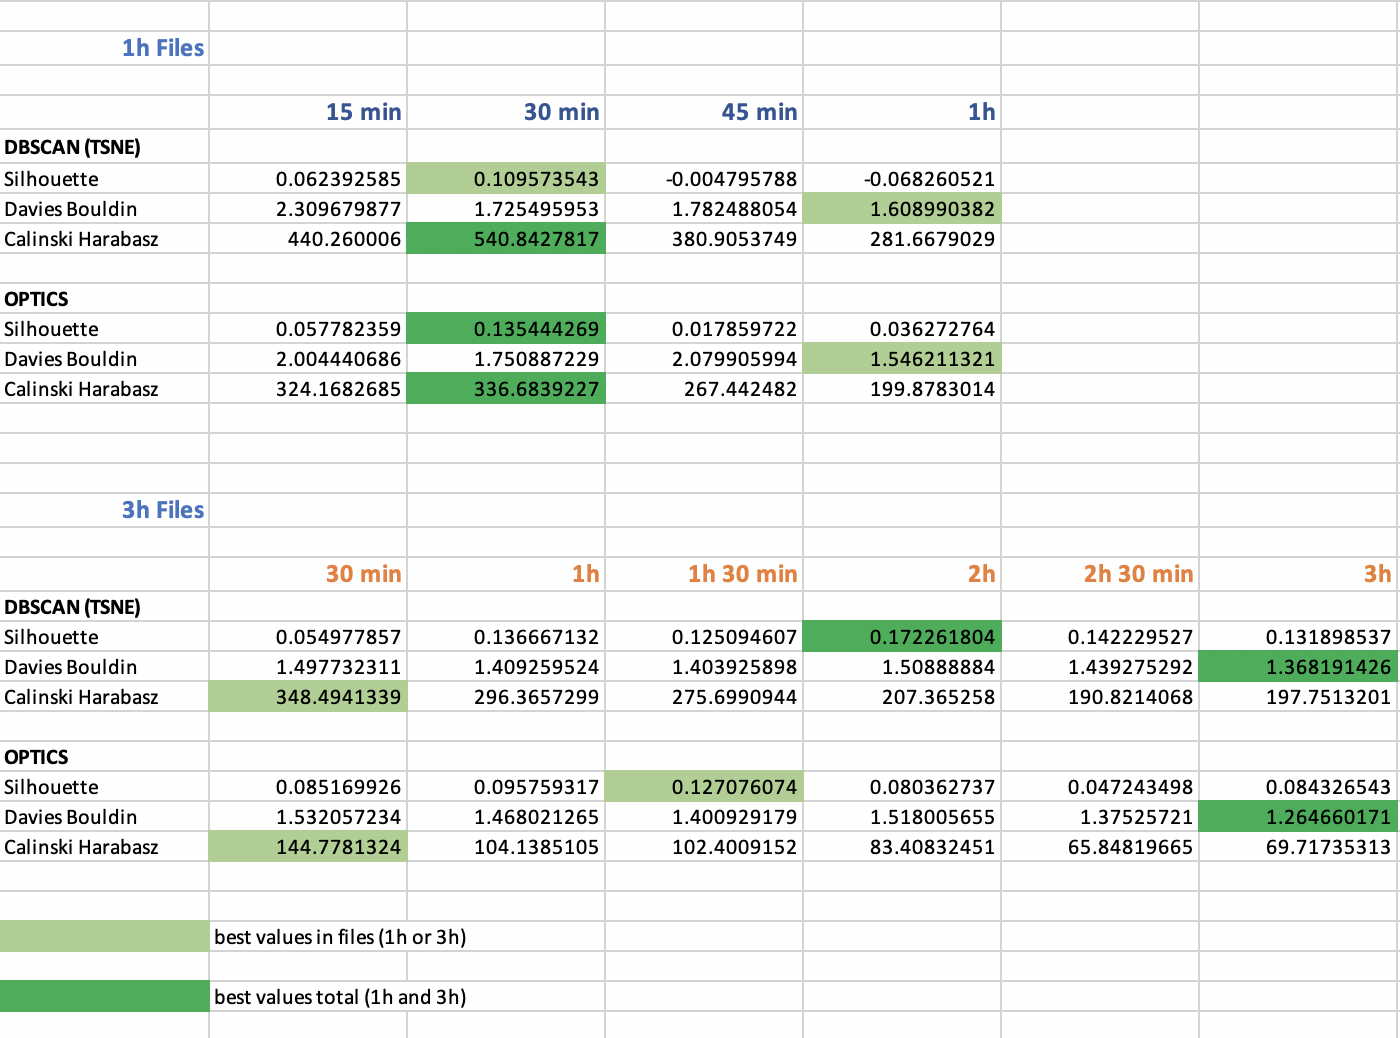
\includegraphics[width=0.8\textwidth]{./images/clusteringResults/clusteringResults5.png}
  \caption{Evaluation scores comparison averaged from 2 runs of t-SNE and clustering with a learning rate of 800.}
  \label{figure:clusteringResults5}
\end{figure}